\documentclass[noauthor,nooutcomes,12pt]{ximera}

\graphicspath{  
{./}
{./whoAreYou/}
{./drawingWithTheTurtle/}
{./bisectionMethod/}
{./circles/}
{./anglesAndRightTriangles/}
{./lawOfSines/}
{./lawOfCosines/}
{./plotter/}
{./staircases/}
{./pitch/}
{./qualityControl/}
{./symmetry/}
{./nGonBlock/}
}


%% page layout
\usepackage[cm,headings]{fullpage}
\raggedright
\setlength\headheight{13.6pt}


%% fonts
\usepackage{euler}

\usepackage{FiraMono}
\renewcommand\familydefault{\ttdefault} 
\usepackage[defaultmathsizes]{mathastext}
\usepackage[htt]{hyphenat}

\usepackage[T1]{fontenc}
\usepackage[scaled=1]{FiraSans}

%\usepackage{wedn}
\usepackage{pbsi} %% Answer font


\usepackage{cancel} %% strike through in pitch/pitch.tex


%% \usepackage{ulem} %% 
%% \renewcommand{\ULthickness}{2pt}% changes underline thickness

\tikzset{>=stealth}

\usepackage{adjustbox}

\setcounter{titlenumber}{-1}

%% journal style
\makeatletter
\newcommand\journalstyle{%
  \def\activitystyle{activity-chapter}
  \def\maketitle{%
    \addtocounter{titlenumber}{1}%
                {\flushleft\small\sffamily\bfseries\@pretitle\par\vspace{-1.5em}}%
                {\flushleft\LARGE\sffamily\bfseries\thetitlenumber\hspace{1em}\@title \par }%
                {\vskip .6em\noindent\textit\theabstract\setcounter{question}{0}\setcounter{sectiontitlenumber}{0}}%
                    \par\vspace{2em}
                    \phantomsection\addcontentsline{toc}{section}{\thetitlenumber\hspace{1em}\textbf{\@title}}%
                     }}
\makeatother



%% thm like environments
\let\question\relax
\let\endquestion\relax

\newtheoremstyle{QuestionStyle}{\topsep}{\topsep}%%% space between body and thm
		{}                      %%% Thm body font
		{}                              %%% Indent amount (empty = no indent)
		{\bfseries}            %%% Thm head font
		{)}                              %%% Punctuation after thm head
		{ }                           %%% Space after thm head
		{\thmnumber{#2}\thmnote{ \bfseries(#3)}}%%% Thm head spec
\theoremstyle{QuestionStyle}
\newtheorem{question}{}



\let\freeResponse\relax
\let\endfreeResponse\relax

%% \newtheoremstyle{ResponseStyle}{\topsep}{\topsep}%%% space between body and thm
%% 		{\wedn\bfseries}                      %%% Thm body font
%% 		{}                              %%% Indent amount (empty = no indent)
%% 		{\wedn\bfseries}            %%% Thm head font
%% 		{}                              %%% Punctuation after thm head
%% 		{3ex}                           %%% Space after thm head
%% 		{\underline{\underline{\thmname{#1}}}}%%% Thm head spec
%% \theoremstyle{ResponseStyle}

\usepackage[tikz]{mdframed}
\mdfdefinestyle{ResponseStyle}{leftmargin=1cm,linecolor=black,roundcorner=5pt,
, font=\bsifamily,}%font=\wedn\bfseries\upshape,}


\ifhandout
\NewEnviron{freeResponse}{}
\else
%\newtheorem{freeResponse}{Response:}
\newenvironment{freeResponse}{\begin{mdframed}[style=ResponseStyle]}{\end{mdframed}}
\fi



%% attempting to automate outcomes.

%% \newwrite\outcomefile
%%   \immediate\openout\outcomefile=\jobname.oc
%% \renewcommand{\outcome}[1]{\edef\theoutcomes{\theoutcomes #1~}%
%% \immediate\write\outcomefile{\unexpanded{\outcome}{#1}}}

%% \newcommand{\outcomelist}{\begin{itemize}\theoutcomes\end{itemize}}

%% \NewEnviron{listOutcomes}{\small\sffamily
%% After answering the following questions, students should be able to:
%% \begin{itemize}
%% \BODY
%% \end{itemize}
%% }
\usepackage[tikz]{mdframed}
\mdfdefinestyle{OutcomeStyle}{leftmargin=2cm,rightmargin=2cm,linecolor=black,roundcorner=5pt,
, font=\small\sffamily,}%font=\wedn\bfseries\upshape,}
\newenvironment{listOutcomes}{\begin{mdframed}[style=OutcomeStyle]After answering the following questions, students should be able to:\begin{itemize}}{\end{itemize}\end{mdframed}}



%% my commands

\newcommand{\snap}{{\bfseries\itshape\textsf{Snap!}}}
\newcommand{\flavor}{\link[\snap]{https://snap.berkeley.edu/}}
\newcommand{\mooculus}{\textsf{\textbf{MOOC}\textnormal{\textsf{ULUS}}}}


\usepackage{tkz-euclide}
\tikzstyle geometryDiagrams=[rounded corners=.5pt,ultra thick,color=black]
\colorlet{penColor}{black} % Color of a curve in a plot



\ifhandout\newcommand{\mynewpage}{\newpage}\else\newcommand{\mynewpage}{}\fi

\usepackage{fullpage}
\makeatletter
%% no number for activity
\newcommand\logostyle{%
  \def\activitystyle{activity-chapter}
  \def\maketitle{%
                {\flushleft\small\sffamily\bfseries\@pretitle\par\vspace{-1.5em}}%
                {\flushleft\LARGE\sffamily\bfseries\@title \par }%
                {\vskip .6em\noindent\textit\theabstract\setcounter{problem}{0}\setcounter{sectiontitlenumber}{0}}%
                    \par\vspace{2em}
                    \phantomsection\addcontentsline{toc}{section}{\textbf{\@title}}%
                     \setcounter{titlenumber}{0}}}
\makeatother
\newcommand{\nameblankgen}{\noindent\textbf{Name(s) (please print):}\ \hrulefill \\

\hrulefill}
\logostyle



\title{Repcount and rainbows}
\author{Bart Snapp}

\begin{document}
\begin{abstract}
  Change your code as you repeat it!
\end{abstract}
\maketitle

\nameblankgen

\begin{multicols*}{2}
  
The command \lc{repeat} might seem pretty cool, but it really comes
alive when you combine it with \lc{repcount}. On the $i$th repetition
of a \lc{repeat} command, the command \lc{repcount} produces the number
$i$. We can use the command \lc{print} to witness this:
\begin{logo}
repeat 10 [ print repcount ]
\end{logo}
This produces a list of numbers, $1$--$10$. The command \lc{print} is
used to figure out values in programs while you write them.  Using
\lc{repcount} we can produce some really cool drawings, especially
when combined with the command \lc{\%}, that means ``take the
remainder,'' like in long division.

\begin{logo}
ht setcolor 0 fill rt 17
repeat 45 [ 
  setwidth .2*repcount 
  setcolor repcount % 15 + 1 
  fd repcount * 15 rt 144 ]
\end{logo}

\begin{logoout}
  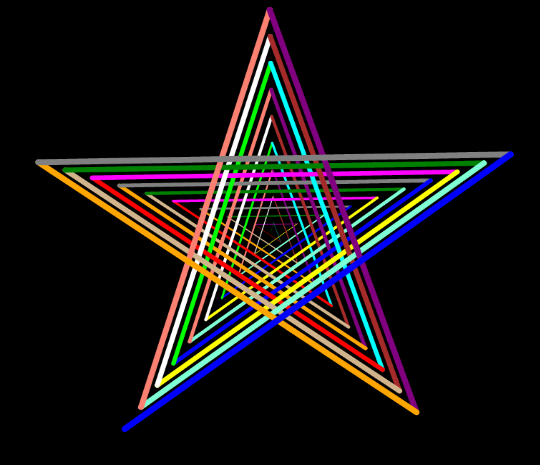
\includegraphics[width=.4\textwidth]{superStar.png}
\end{logoout}


Now we will use \lc{repeat} and \lc{repcount} to produce a picture of
the Sun.
\begin{logo}
ht setcolor [ 10 10 30 ] fill
to rays
  repeat 12 [ pu fd 120 pd
  repeat 100 [
    setwidth 14-14*repcount/(100) fd 1.2 ]
  pu bk 240 rt 30 ]
end
repeat 6 [ rt 41
  setcolor pick [ 4 6 14 ] rays ]
setcolor 6
filled 6 [ circle ]
\end{logo}
If you remember to define \lc{circle}, it makes:
\begin{logoout}
  
\includegraphics[width=.4\textwidth]{sun.png}
\end{logoout}


\section{Commands to know}
\begin{tabular}{lll}
  \lc{CMD}   & Description                 \\ \hlinewd{1pt}
  \lc{repcount} & tells you which repetition  \\
  \lc{print \#}     & prints \lc{\#}\\
  \lc{:n \% :d} & remainder of \lc{:n} divided by \lc{:d} 
\end{tabular}


\end{multicols*}

\newpage

\begin{problem}
  Above, we introduce the command \lc{\%} but we do not explain it
  very well. Can you explain the command \lc{\%}? Note, this command
  is sometimes called ``mod.''
\end{problem}

\mynewpage

\begin{problem}
  Sometimes you want \textit{nested} repcounts.  Use \lc{repcount} to
  help you make a command that will make rainbows.  Show-off your work
  with your code and a picture.
\end{problem}

\mynewpage

\begin{problem}
  Create a picture involving a rainbow, clouds, and the Sun in the
  sky. Show-off your work with your code and a picture.
\end{problem}

\mynewpage

\begin{problem}%http://fmslogo.sourceforge.net/workshop/basic-loops.shtml
  Here's some code I found lying around the interwebs:
\begin{logo}
repeat 100 [
  fd repcount * 2 rt 91 ]
\end{logo}
  Use \lc{repcount} to help you make it awesome! Show-off your work
  with your code and a picture.
\end{problem}



\mynewpage

\begin{problem}
Here's some code I found lying around the interwebs:
\begin{logo}
repeat 20 [
  repeat 180 [
    fd 4 rt 2 ]
  rt 18 ]
\end{logo}
Use \lc{repcount} to help you make it awesome! Show-off your work with
your code and a picture
\end{problem}


\end{document}
